\section{Einleitung}
	\label{sec:einleitung}
	In diesem Versuch soll der Wirkungsgrad einer Solarzelle bestimmt werden.
	Durch Messung von Strom und Spannung und mit Kenntniss der Intensit"at des einfallenden Lichtes l"asst sich dieser bestimmen.


\section{Theorie und Hintergrund}
	\label{sec:theorie}

	\subsection{Aufbau und Funktion einer Solarzelle}
		\label{subsec:aufbau_funktion}
		Eine Solarzelle ist grunds"atzlich aufgebaut wie eine Diode.
		Eine p- und n-dotierte Halbleiterschicht werden zusammengebracht, wodurch am Grenzbereich ein starkes elektrisches Feld entsteht.

		Wird in diesem Bereich ein Photon absorbiert, das gen"ugend Energie besitzt um den Bandabstand des Atoms zu "uberschreiten, entsteht ein Elektron -- Loch Paar.
		Auf Grund des elektrischen Feldes, kann das Paar nicht sofort rekombinieren und Elektron und Loch werden abtransportiert.

		"Uber Kontakte an den Halbleiterschichten k"onnen die Ladungstr"ager dann zu einem Strom beitragen, der durch den Verbraucher abflie"st und dabei Arbeit verrichtet.

		\begin{figure}[h]
			\centering
			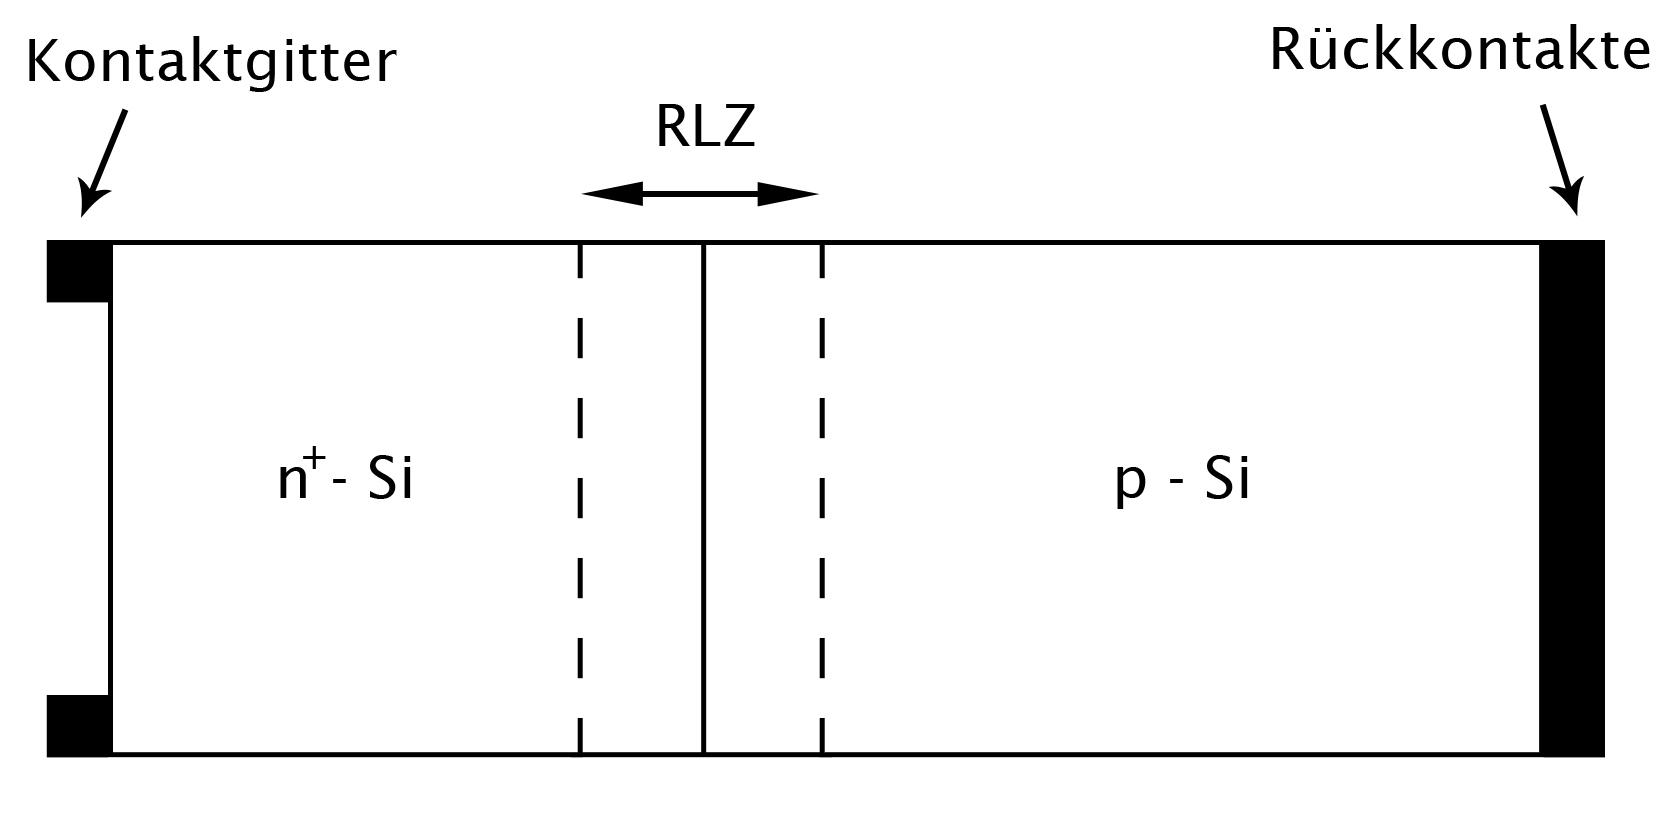
\includegraphics[width = 15cm]{img/diode_neu.jpg}
			\caption{Schematischer Aufbau einer Solarzelle}
			\label{fig:diode}
		\end{figure}

	\subsection{Technische Umsetzung}
		\label{sub:umsetzung}
		Als Rohstoff f"ur die meisten Solarzellen dient Silizium.
		Es kann g"unstig verarbeitet werden und der Umgang mit diesem Stoff ist gut erforscht.
		Nachdem in den letzten Jahrenzehnten zun"achst monokristallines und sp"ater multikristallines Silizium (c-Si) verwendet wurde,
		versucht man heute, die Effizienz von amorphen Silizium (a-Si) zu erh"ohnen, um dieses marktf"ahig zu machen.

		Bei c-Si geht w"ahrend der Herstellung der Wafer viel n"amlich Material verloren, was die Kosten steigen l"asst.
		Wafer aus a-Si k"onnen dagegen nahezu verlustfrei hergestellt werden.
		Au"serdem ist a-Si -- Im Gegensatz zu c-Si, was zun"achst dotiert werden muss -- ein direkter Halbleiter.
		Der Wirkungsgrad $\eta$ von a-Si ist jedoch noch zu gering um es wirtschaftlich nutzen zu k"onnen.

	\subsection{Berechnung des Wirkungsgrades $\eta$}
		\label{subsec:wirkungsgrad}
		F"ur den Wirkungsgrad $\eta$ der Zelle ist das Verh"altnis aus entnommener Leistung $P_\mathrm{max}$ und einfallender Leistung $P_\mathrm{ein}$ entscheidend.

		Es gilt

		\begin{equation}
			\eta = \frac{P_\mathrm{max}}{P_\mathrm{ein}} = \frac{U_\mathrm{o} I_\mathrm{k} F}{P_\mathrm{ein}} .
		\end{equation}

		Hier bezeichnet $U_\mathrm{o}$ die Spannung bei offenem Stromkreis und $I_\mathrm{k}$ den Kurzschlussstrom. Der F"ullfaktor $F$ bezeichnet das Verh"altnis der maximalen Fl"ache unter der I-U-Kennlinie zur Fl"ache $I_\mathrm{k} \cdot U_\mathrm{o}$.